\documentclass{article}
\usepackage{graphicx}
\usepackage{float}
\usepackage{hyperref}  % 导入 hyperref 包

\title{License Plate Recognition Process Description}
\begin{document}
	\maketitle
	Github rep with code address \href{https://github.com/chenjunbo/mse803}
	
	\section{Overall Process}
	The overall process is mainly divided into two major steps:
	\begin{enumerate}
		\item Use multiple algorithms to extract the outline of the license plate, obtain the license plate cut-out from the original image according to the outline, and use the SVM algorithm model to determine whether the cut-out is a license plate.
		\item Determine the color of the license plate based on the license plate cut-out, and use the contour extraction algorithm to extract the license plate character outline. Obtain the license plate cut-out from the binary image according to the outline. Use the ANN algorithm model with the Chinese character model, blue license plate model, and green license plate model to recognize the text content of the character cut-out.
	\end{enumerate}
	
	\begin{figure}[H]
		\centering
		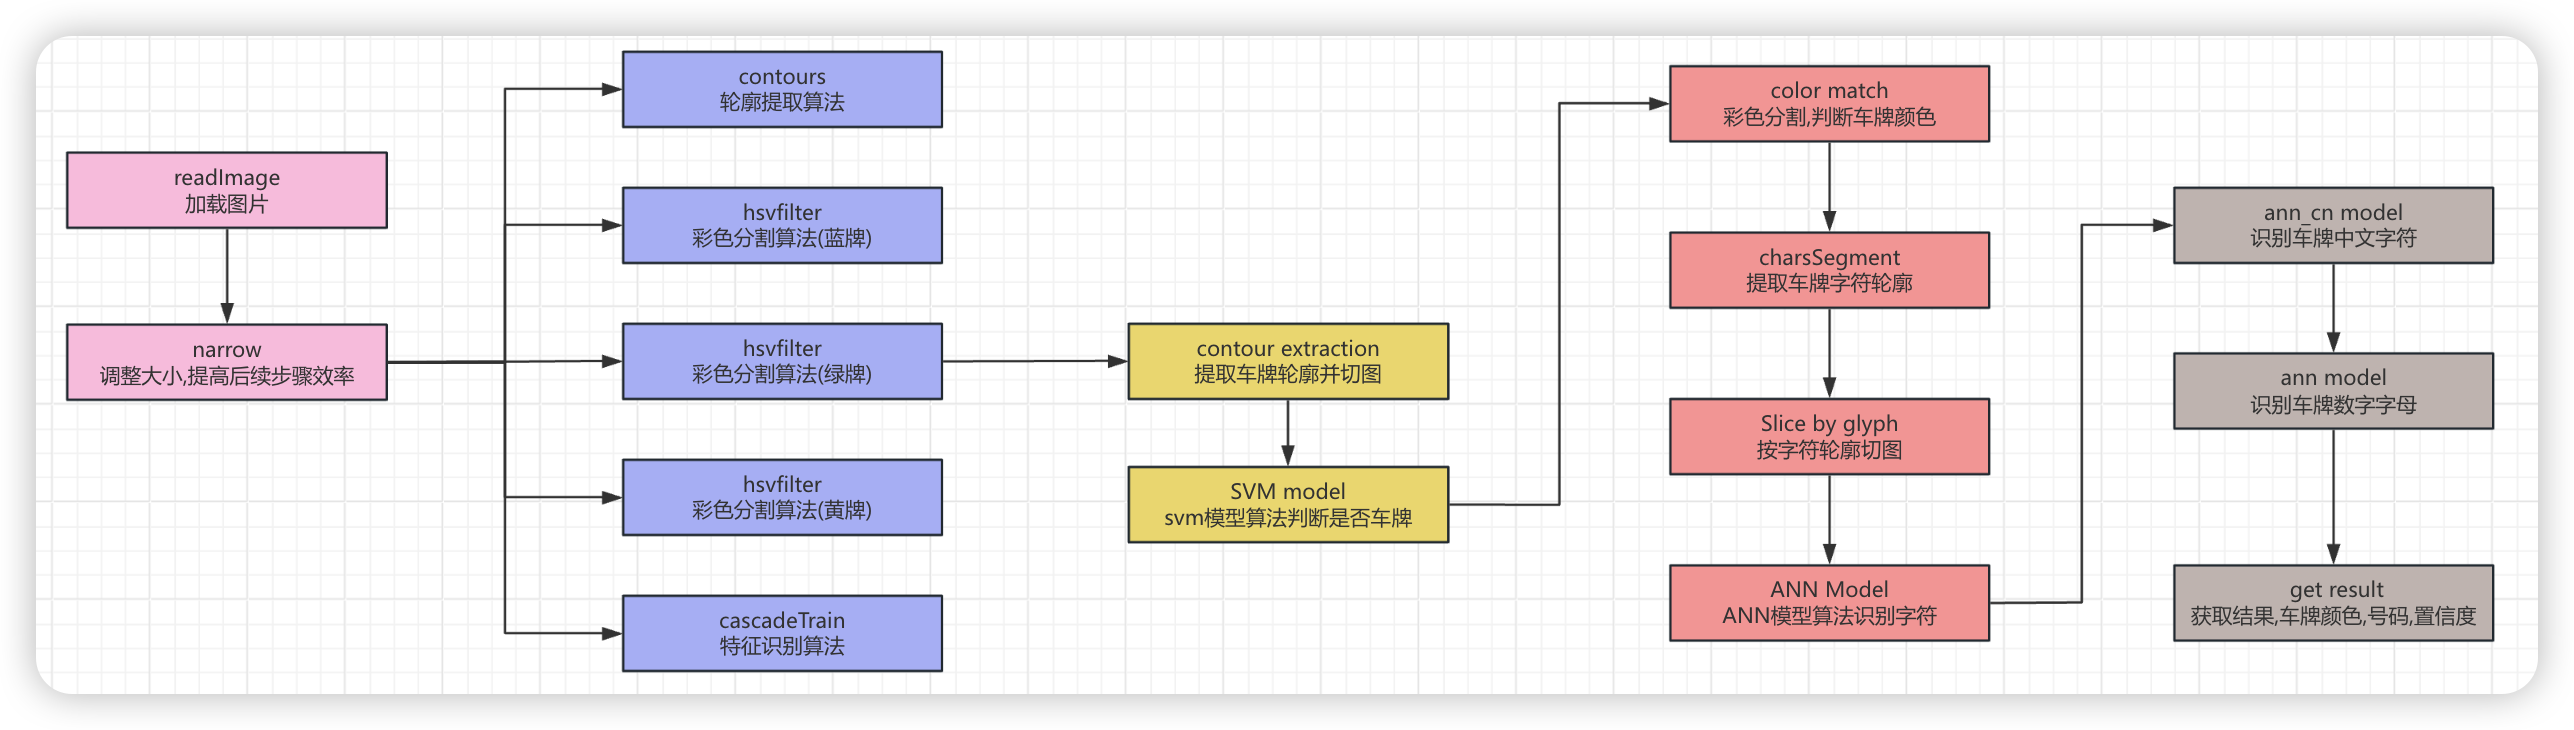
\includegraphics[width=\linewidth]{mdpic/image-20240925000409837.png}
		\caption{License Plate Recognition Example}
	\end{figure}
	
	\section{License Plate Block Extraction}
	The purpose is to extract the block containing the license plate from the license plate image. There are three implementation methods:
	\begin{enumerate}
		\item Contour extraction algorithm
		\item Color segmentation extraction algorithm
		\item Feature recognition extraction algorithm
	\end{enumerate}
	
	\begin{figure}[H]
		\centering
		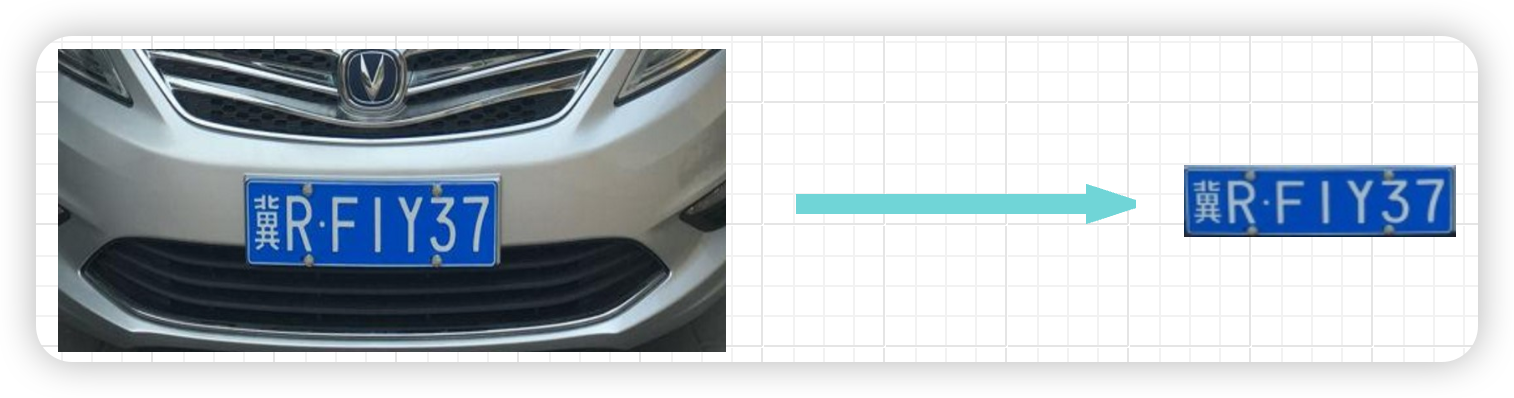
\includegraphics[width=\linewidth]{mdpic/image-20240924224339600.png}
		\caption{Block Extraction Example}
	\end{figure}
	
	\subsection{Contour Extraction Algorithm}
	The main image processing process is as follows:
	\begin{figure}[H]
		\centering
		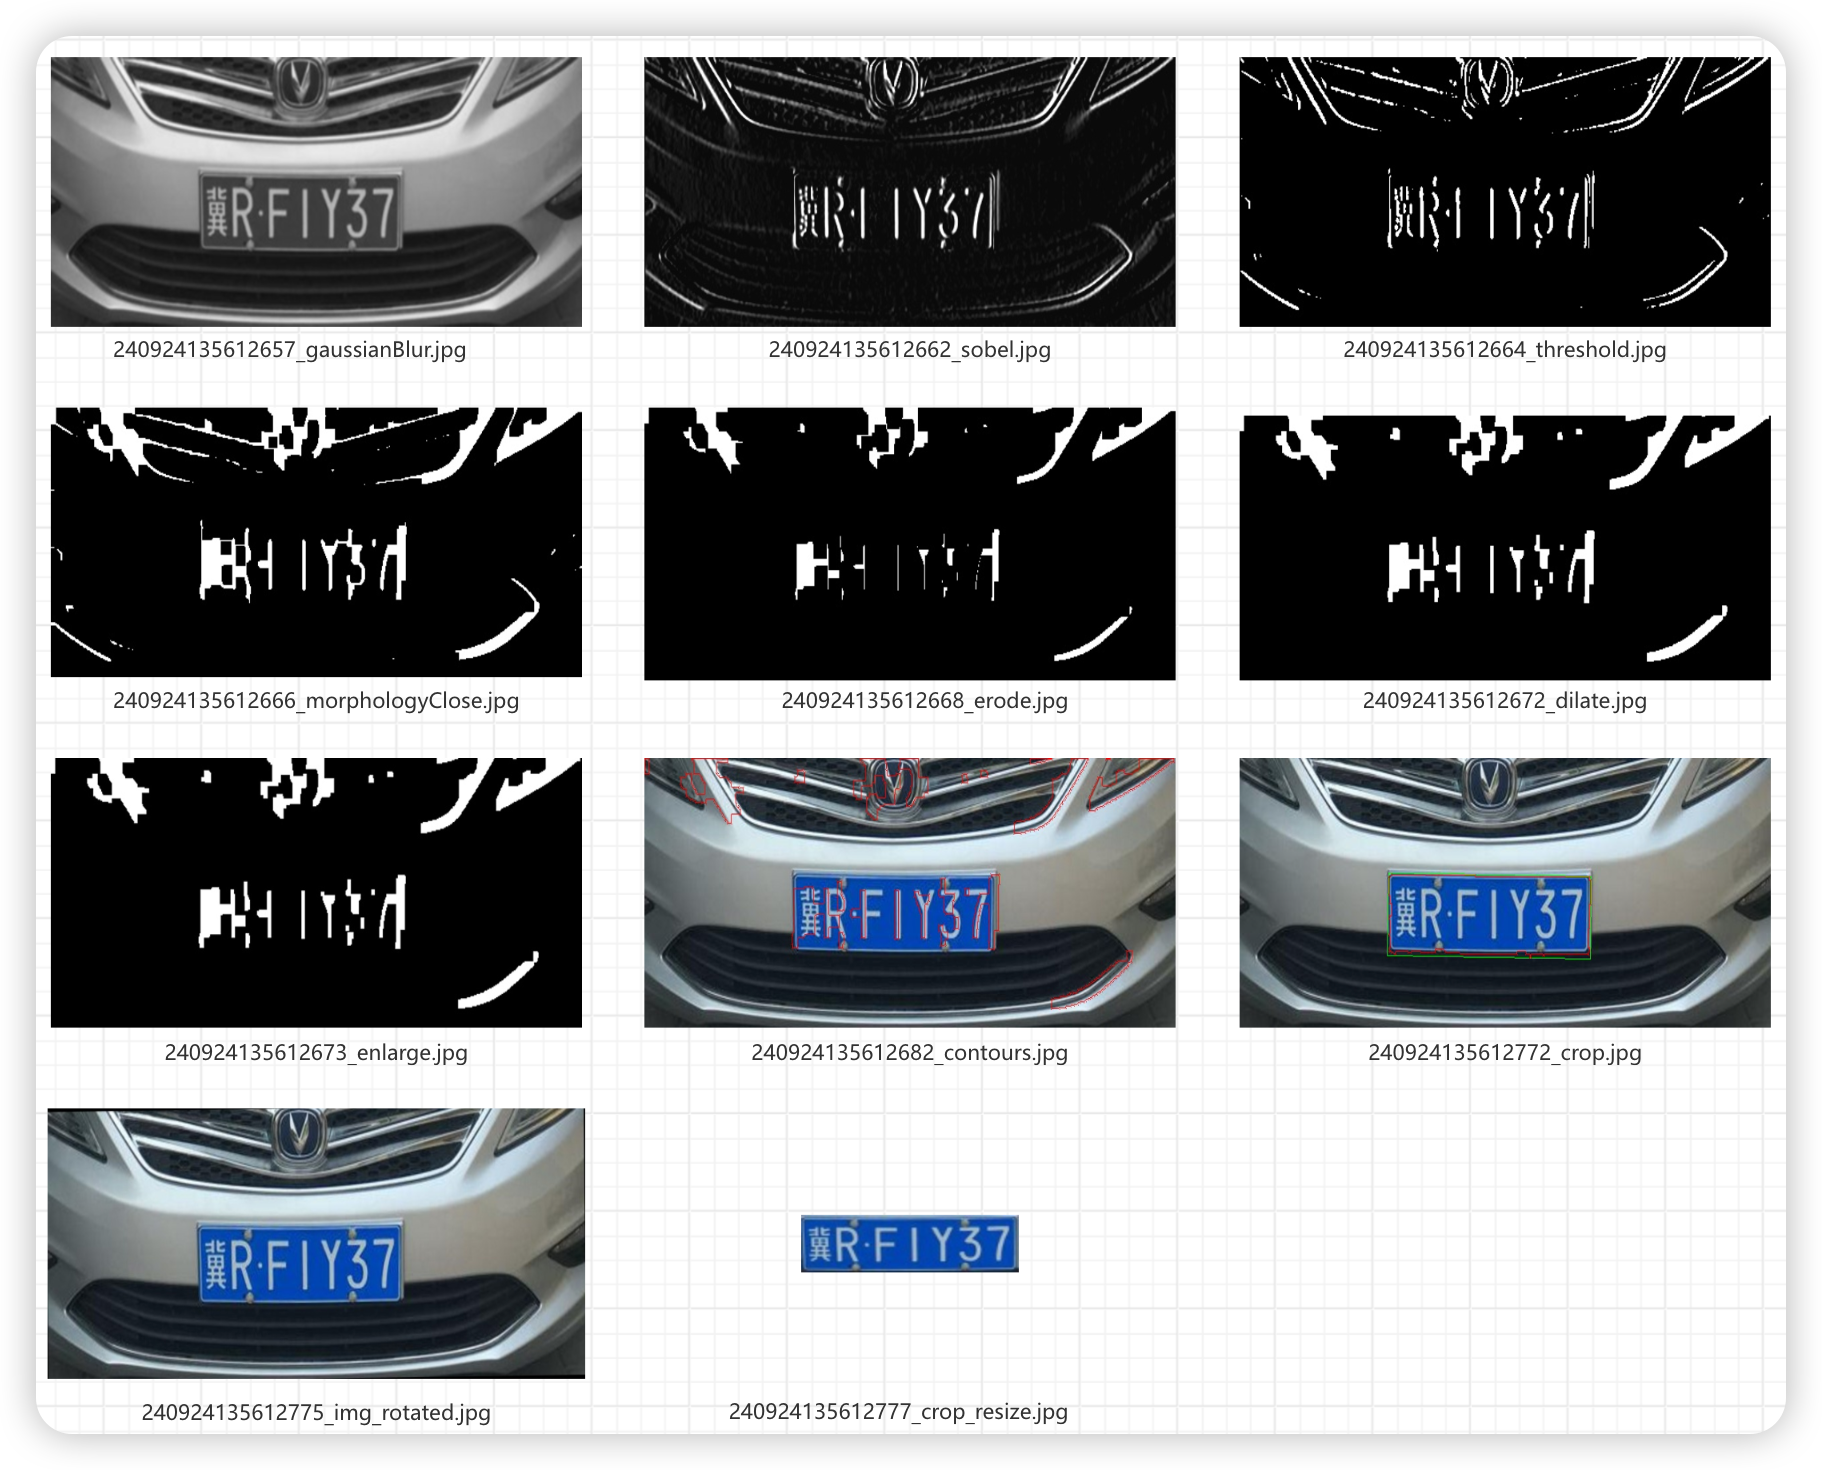
\includegraphics[width=\linewidth]{mdpic/image-20240924225915405.png}
		\caption{Contour Extraction Example}
	\end{figure}
	
	\begin{enumerate}
		\item Read the image, resize it, and then grayscale the image.
		\item Apply Gaussian blur to remove noise.
		\item Perform Sobel operation to detect image edges.
		\item Binarize the image, converting edges to white (value 255) and other content to black (value 0).
		\item Perform image closing operation to merge adjacent edge lines into blocks.
		\item Apply edge erosion to remove small connecting lines and separate large block areas.
		\item Perform edge expansion to restore the block areas affected by erosion.
		\item Resize the image to the original size, extract the contour according to the binary image.
		\item Cut the image from the original image based on the extracted contour.
		\item Adjust the cut image to a fixed size: 136x36 pixels, for the SVM algorithm to determine whether it is a license plate.
	\end{enumerate}
	
	The above steps include some additional steps like contour screening and image rotation correction. This method is general-purpose, and adjusting some parameters can significantly increase accuracy in specific scenarios.
	
	\subsection{Color Segmentation Extraction Algorithm}
	The main image processing process is as follows:
	
	\begin{figure}[H]
		\centering
		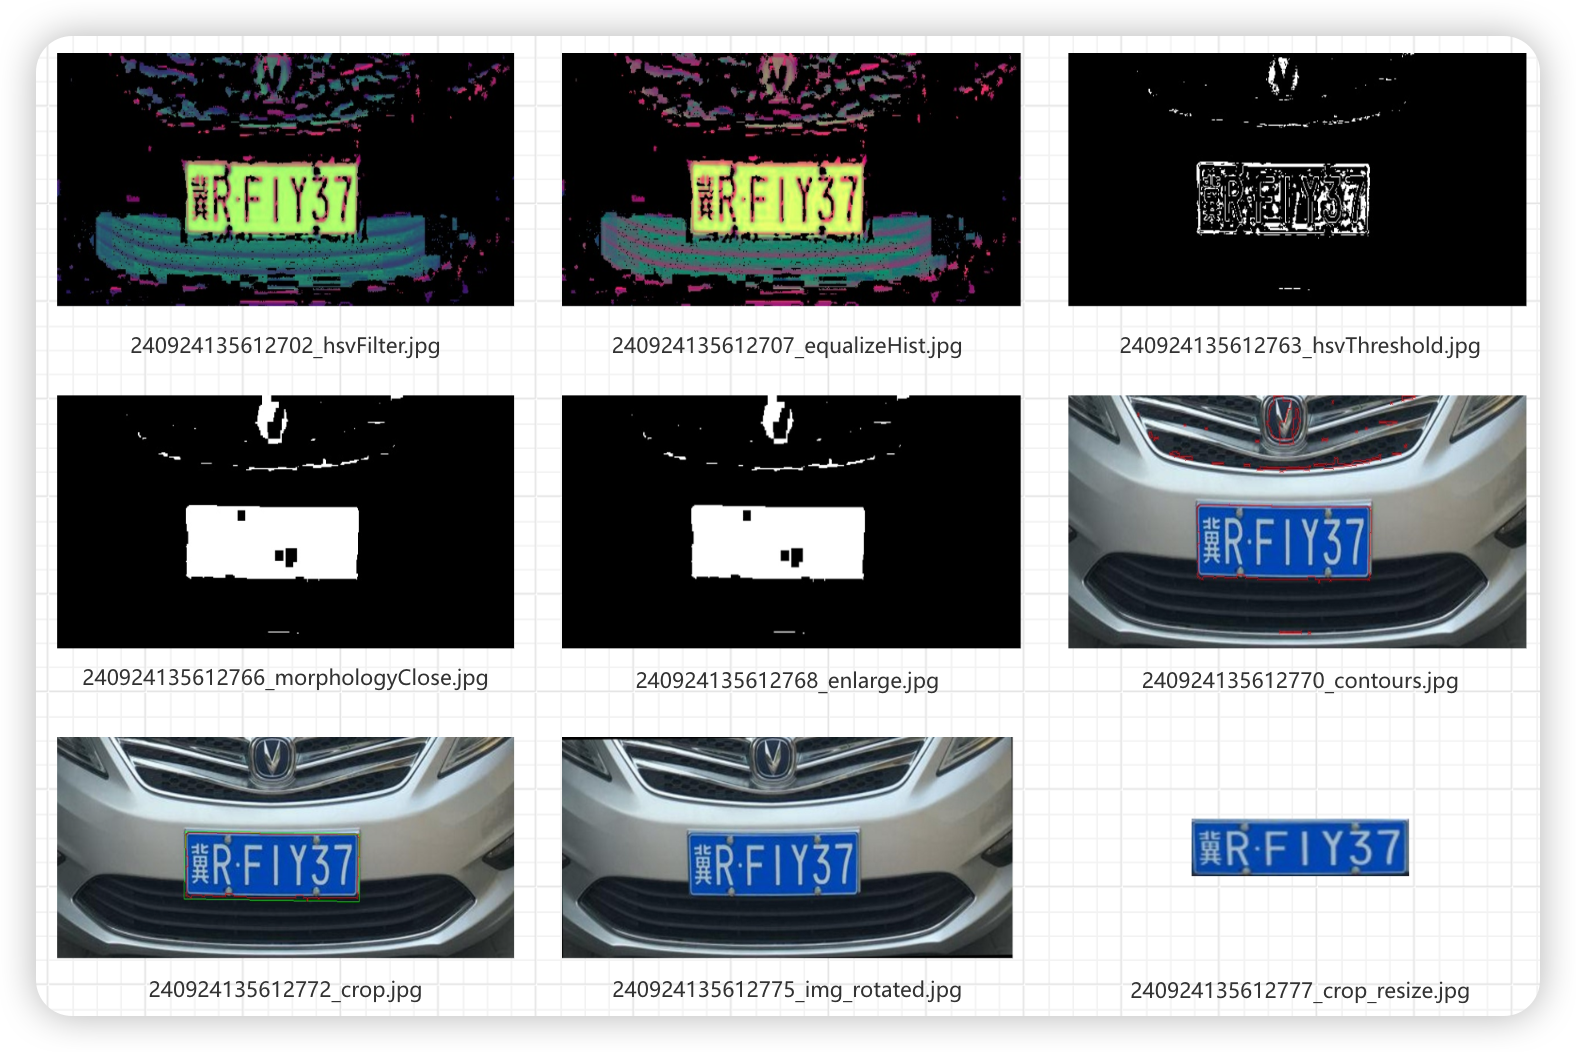
\includegraphics[width=\linewidth]{mdpic/image-20240924230824445.png}
		\caption{Color Segmentation Example}
	\end{figure}
	
	\begin{enumerate}
		\item Convert the image to HSV color space, filter the HSV value range (this range can be located using a color cutting tool).
		\item For blue, green, and yellow plates, the HSV value range differs slightly.
		\item Equalize the image to enhance contrast.
		\item Binarize the image to get the license plate area.
		\item Perform image closing operation to connect the license plate area.
		\item Restore the image to its original size, extract the contour based on the binary image.
		\item Cut the image based on the extracted contour.
		\item Adjust the cut image to a fixed size: 136x36 pixels, for the SVM algorithm model to determine whether it is a license plate.
	\end{enumerate}
	
	This method also includes some extra steps like contour screening and image rotation correction, and it is highly accurate in specific scenarios.
	
	\subsection{Feature Recognition and Extraction Algorithm}
	The main image processing process is as follows:
	
	\begin{figure}[H]
		\centering
		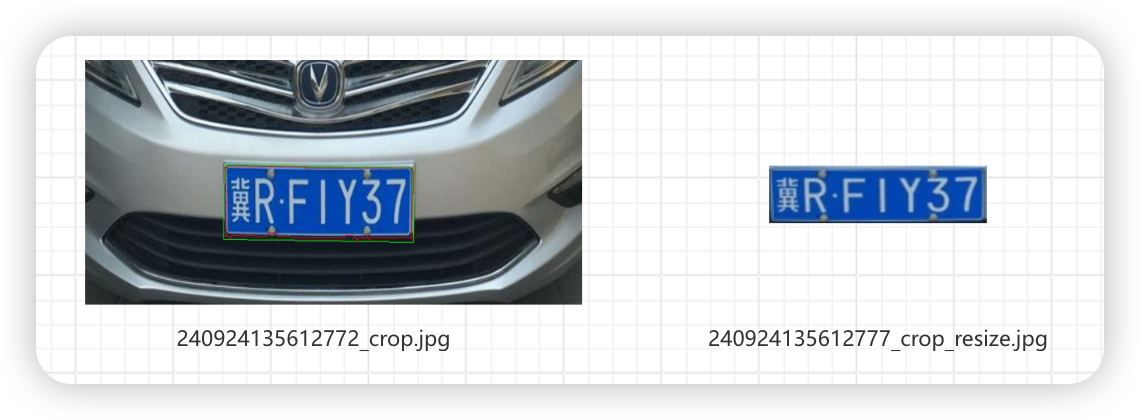
\includegraphics[width=\linewidth]{mdpic/image-20240924230957298.png}
		\caption{Feature Recognition Example}
	\end{figure}
	
	\begin{enumerate}
		\item Use the Haarcascade model to directly identify the position of the license plate and extract the tile cut-out.
		\item Adjust the obtained cut-out to a fixed size: 136x36 pixels, for the SVM algorithm to determine whether it is a license plate.
	\end{enumerate}
	
	This method is widely used, and face recognition often relies on this method. Many feature recognition algorithms exist, but the Haarcascade algorithm is relatively old-fashioned.
	
	\section{License Plate Character Recognition}
	The purpose is to identify the color and number of the license plate from the block.
	
	\begin{figure}[H]
		\centering
		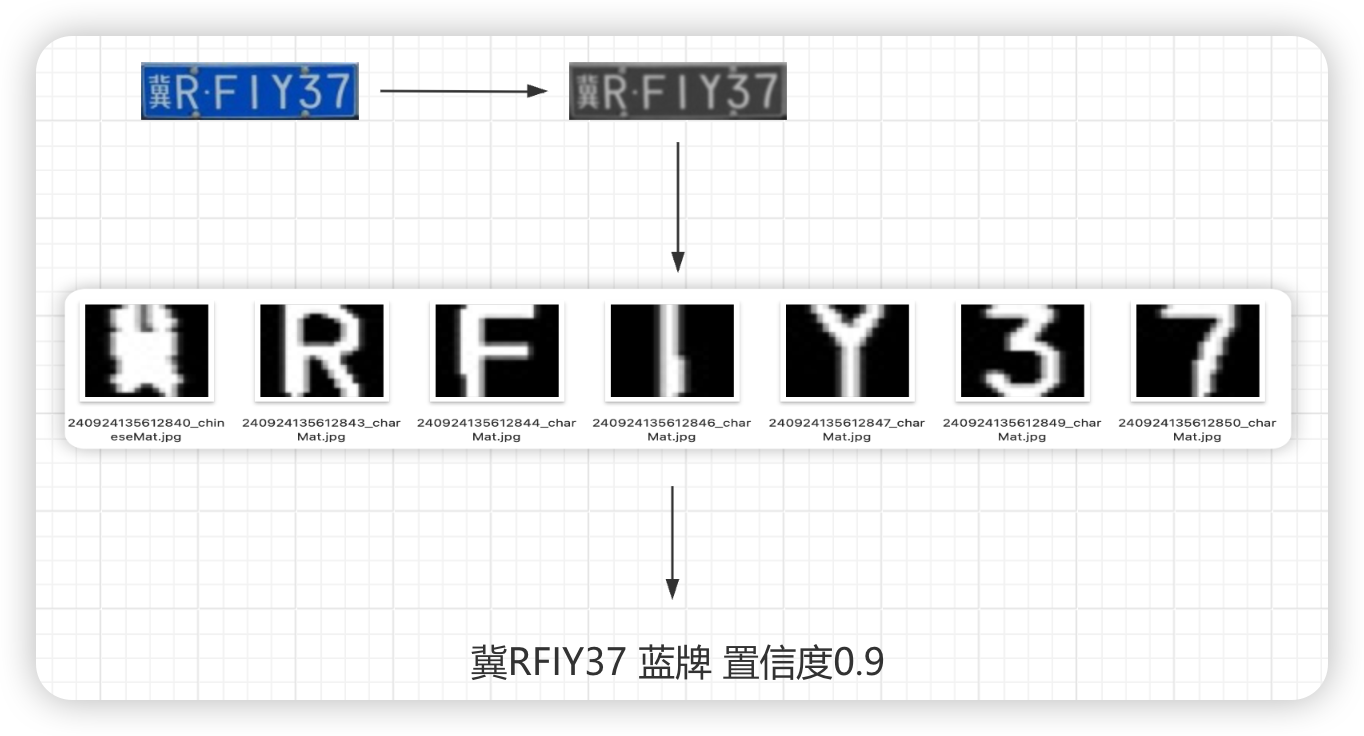
\includegraphics[width=\linewidth]{mdpic/image-20240924232836851.png}
		\caption{Character Recognition Example}
	\end{figure}
	
	\subsection{Image Debugging Process}
	\begin{figure}[H]
		\centering
		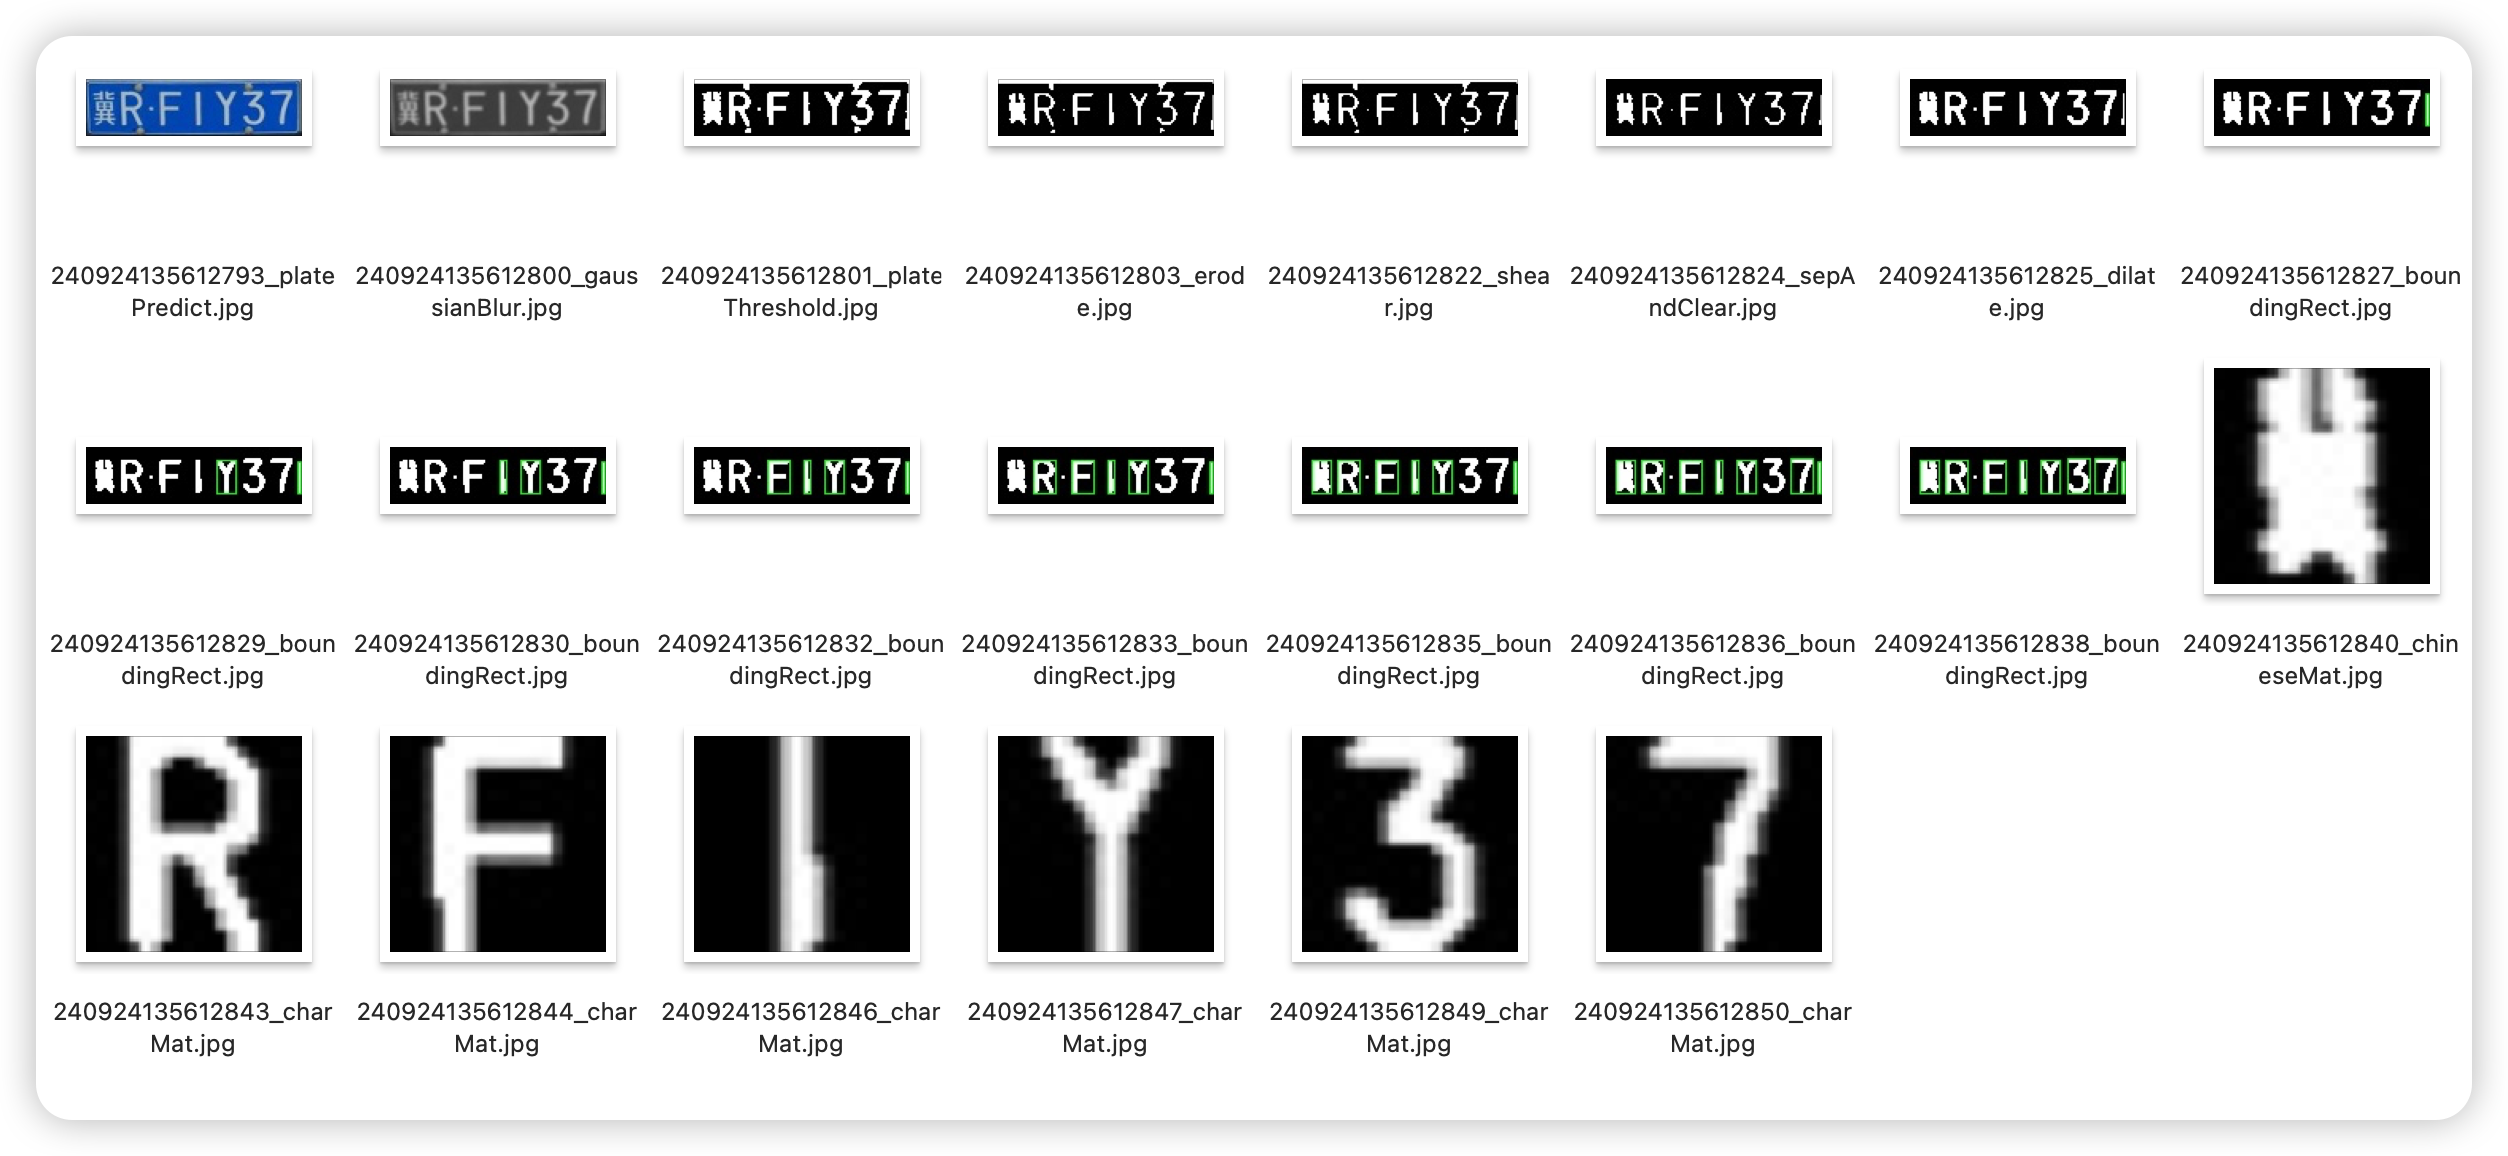
\includegraphics[width=\linewidth]{mdpic/image-20240924231544091.png}
		\caption{Image Debugging Example}
	\end{figure}
	
	\begin{enumerate}
		\item Use the SVM model algorithm to determine whether the block is a license plate.
		\item Convert the block to HSV color space, and after equalizing the image, calculate the license plate color based on the HSV value range and proportion.
		\item Grayscale and Gaussian blur the original image.
		\item Binarize the image; typically, license plates contain only two colors.
		\item Apply edge erosion and expansion.
		\item Perform horizontal or vertical projection to remove borders, rivets, etc.
		\item Correct miscuts.
		\item Extract contours, adjust position, size, and filter contours.
		\item Extract character blocks, resize them to 20x20 pixels, and use the ANN algorithm to recognize the characters, calculate confidence, etc.
	\end{enumerate}
	
\end{document}